\chapter{LABoratories}

\section{First LAB}
\cite{LAB1}

\subsection{Software Tools}
\begin{table}[H]
    \centering
    \begin{tabular}{|p{3cm}|p{7cm}|}\hline
        \rowcolor{gray!30}
		\textbf{Tool} & \textbf{Description}  \\ \hline
		nmap
			& It is designed to perform quick scanning of large networks.
			\\ \hline
        Ettercap
			& Allows performing man-in-the-middle (MITM) attacks and sniffing attacks in a Local Area Network (LAN).
			\\ \hline
        Wireshark 
            & Allows to capture network traffic.
            \\ \hline
        GVM 
            & Performs vulnerability scanning.
            \\ \hline
    \end{tabular}

    \caption{Main Software Tools}

    \label{tab:mainSoftwareTools}
\end{table}

\begin{table}[H]
    \centering
    \begin{tabular}{|p{3cm}|p{7cm}|}\hline
        \rowcolor{gray!30}
		\textbf{Command} & \textbf{Description} \\ \hline
		Apache2
			& Web server.
			\\ \hline
        VSFTP
			& FTP server.
			\\ \hline
        SSH2
            & SSH server
            \\ \hline
        Exim
            & Mail server
            \\ \hline
    \end{tabular}

    \caption{Additional Software Tools}

    \label{tab:additionalSoftwareTools}
\end{table}

\clearpage
\subsection*{Commands for Softwares}
\begin{table}[H]
	\centering
    \begin{tabular}{|p{6cm}|p{5cm}|p{4cm}|}\hline
        \rowcolor{gray!30}
		\textbf{Command} & \textbf{Description} & \textbf{Options} \\ \hline
		
        sudo systemctl [options] apache2
            & Configuration of server ports are at: \newline /etc/apache2/ports.confs
            & start; stop; restart
        \\ \hline

        systemctl [options] vsftpd
            & Configuration of server ports are at: \newline /etc/vsftpd.conf
            & start; stop; restart
        \\ \hline

        sudo systemctl [options] ssh \newline \newline \textbf{Before starting the server the first time you must generate the keys of the host with the command:}\newline \texttt{ssh-keygen -A}
            & Configuration of server ports are at: \newline /etc/ssh/sshd\_config
            & start; stop; restart
        \\ \hline

        sudo systemctl [options] exim4
            & Configuration of server ports are at: \newline /etc/default/exim4.
            & start; stop; restart
        \\ \hline

        sudo wireshark 
            & Network analyzer 
            & 
        \\ \hline

    \end{tabular}

    \caption{Softwares Commands}

    \label{tab:softwareCommands}
\end{table}

\subsection{Commands for Networking}
\begin{table}[H]
	\centering
    \begin{tabular}{|p{6cm}|p{3cm}|p{6cm}|}\hline
        \rowcolor{gray!30}
		\textbf{Command} & \textbf{Description} & \textbf{Options} \\ \hline
		
        arp 
            & Manipulets the system ARP cache.
            & -d(elete) <ipAddr>; 
                \newline Show: -e (fixed); -a 
        \\ \hline

        ip 
            & Analyse and manipulate the routing of IP packets
            & neigh flush all (delete);
                \newline -s -s neigh flush all (all-verbose)
        \\ \hline

        netstat
            & Displays detailed information about a network.
            & -l(istening) \newline -t(cp); -u(dp)
        \\ \hline

        nmap <ipAddrVictim>
            & Obtain information of a victim in the network
            & -O(S); -sT(CP); -Pn (ping)
                \newline -p <port>; 
                \newline -v(erbose); -sV (service/Version)
                \newline -T<num> (timer 0-6)
                \newline -A(ggressive)
        \\ \hline

        ettercap \newline \newline configuration files: \newline \texttt{man etter.conf} \newline \texttt{/etc/ettercap/etter.conf}.
            & Executes man-in-the-middle attacks in a LAN.
            & -T(ext UI); -q(uiet)
            \newline -M(ITM) [arp;icmp;dhcp;port]
            \newline -e "<regExpr>"
            \newline -L <logFile>; -P(lugin)
        \\ \hline

        s-nail 
            & Mail Client. Send and receive Internet mail
            & -s(ubject); -S(et var)
        \\ \hline


    \end{tabular}

    \caption{Network Commands}

    \label{tab:basicNetworkCommands}
\end{table}
\clearpage

\subsection*{Insights}
\begin{itemize}
	\item Network Fingerprinting allows obtaining information on the remote host’s operating system. Possible using the tool nmap. This technique is based on the fact that different types of operating systems implement differently the TCP/IP stack \textrightarrow nmap.
	\item The technique known as Port Scanning is used to obtain information about which ports of a particular host are open \textrightarrow nmap.
    \item A special expression can be used with the port parameter as \texttt{-p <initial>-<ending>}
    \item Identification of services \textrightarrow nmap or a vulnerabilities scanner like GVM (Uses an in-depth scanning).
    \item MITM attacks (like ARP poisoning) \textrightarrow ettercap.
\end{itemize}

\subsection*{Commands from the Text}

\begin{lstlisting}[style=bashStyle]
    #FINGERPRINTING
    #Bob(attacker) tries to establish a TCP connection (-sT) on the port 80 (-p 80) of the target host Alice, in order to obtain information about the operating system (-O) running on the victim's machine
    nmap -sT -p 80 -O -v <ipAddrVictim>

    #PORT SCANNING
    #the attacker wants to scan ports of the victim that use tcp connections. Scan the first 1024 ports
    nmap -sT -p 1-1024 -v <ipAddrVictim>
    #version with ping interaction
    nmap -Pn -p 1-1024 -v <ipAddrVictim>

    #IDENTIFICATION of SERVICES
    #the attacker wants to identify the (application) services running on the open ports on victims's machine
    nmap -sV -Pn -p 1-1024 -v <ipAddrVictim>
    #or a more aggressive version:
    nmap -sV -A -Pn -p 1-1024 -v <ipAddrVictim>
    #-A: Enable OS detection, version detection, script scanning, and traceroute
    #more information are provided on the target machine!!

    #ARP poisoning
    ettercap -Tq -M arp /<ipAddrVictim1>// /<ipAddrVictim2>//
    #in addition with regular expression
    ettercap -Tq -M arp /<ipAddrVictim1>// /<ipAddrVictim2>// -e "<regExpr>"

\end{lstlisting}

\clearpage
\subsubsection{How to use Mail Server - exim}

    \begin{lstlisting}[style=bashStyle]
        #mail server configuration
        dpkg-reconfigure exim4-config

        #start the mail server
        sudo systemctl start exim4

        #another user sends an e-mail to the mail server
            #follow the configuration details reported below
        #all on the same line
        s-nail -S mta=smtp://10.0.24 -S 'from=<userMittent> \\ @kali' -s "<subjectText>" <userReceiver>@kali
        #press enter when finished and then ctrl-D
        
        
    \end{lstlisting}
\begin{figure}[H]
    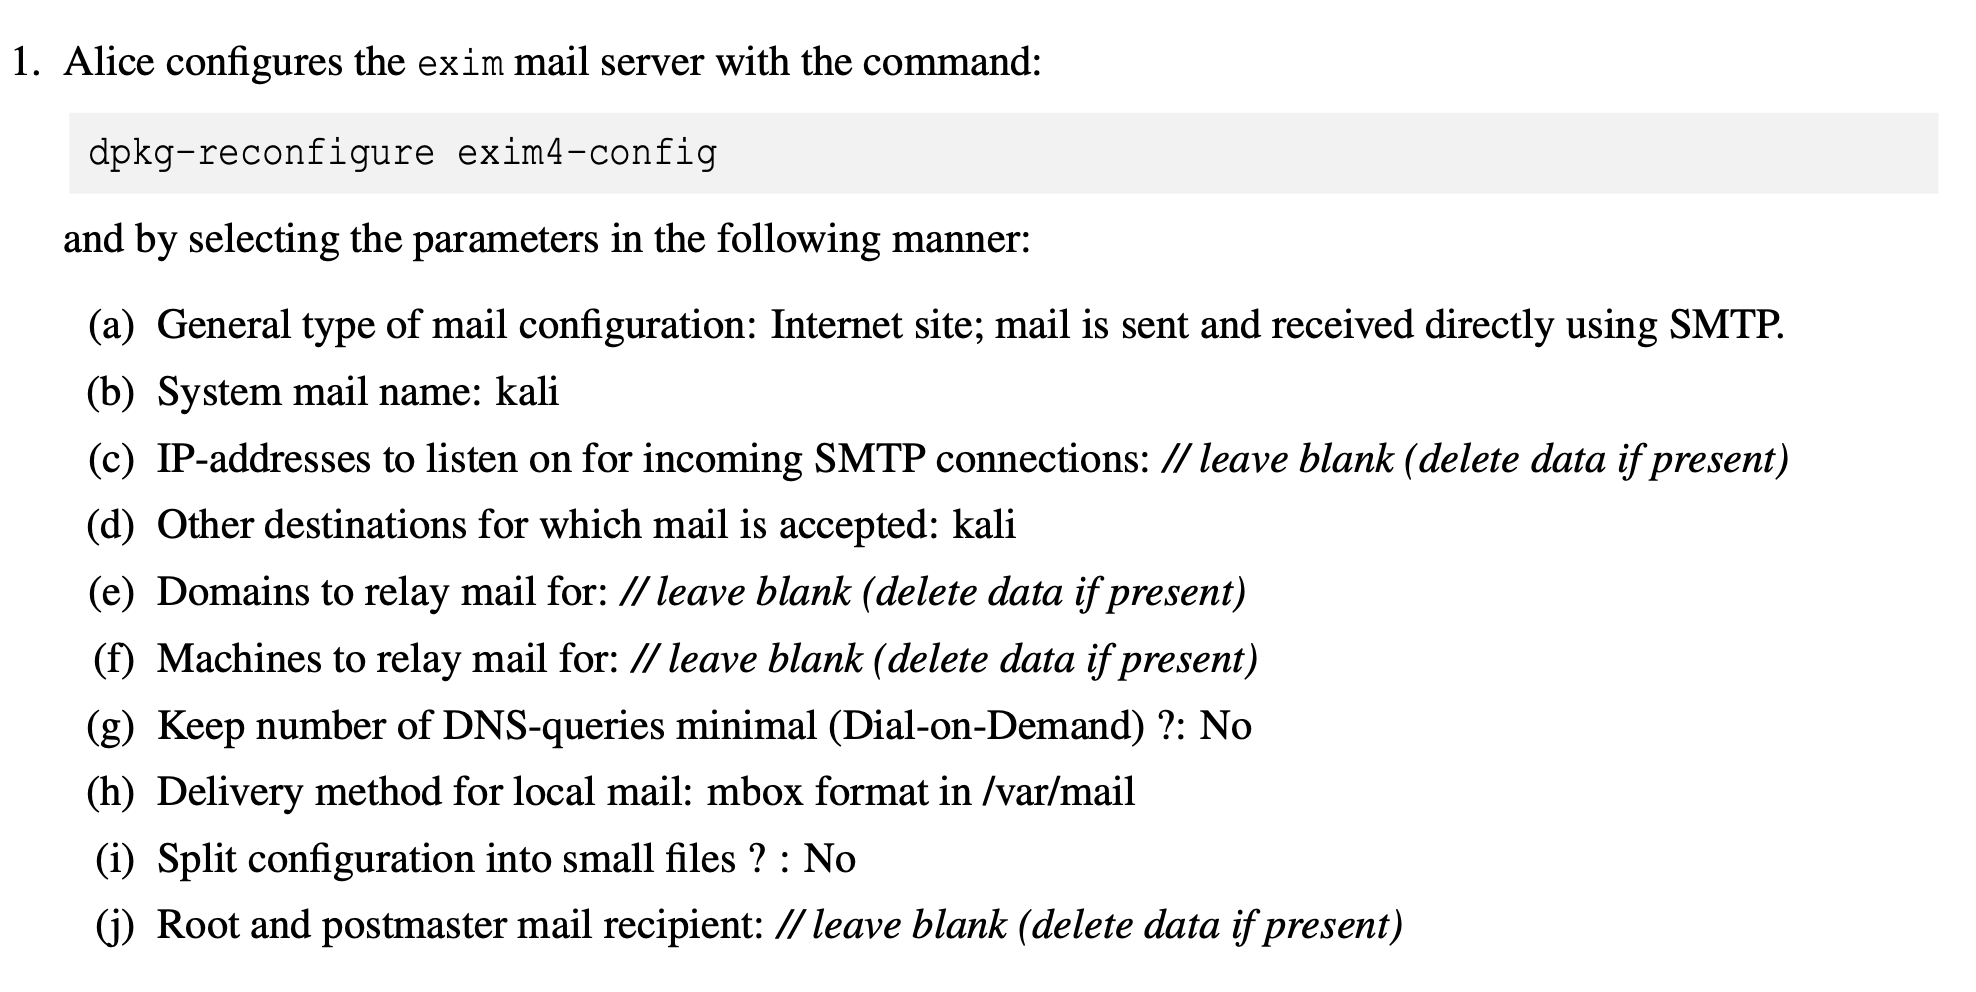
\includegraphics[width=\linewidth]{Images/LABs/exim4config.png}

    \caption{Configuration parameters for exim mail server in the LAB}
    \label{fig:exim4configuration}
    
\end{figure}

\clearpage
